
\subsubsection{NoiseMiner View}

\begin{figure}[!h]
\center
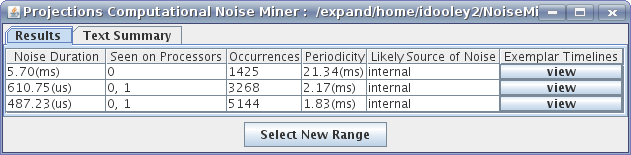
\includegraphics[width=6.0in]{fig/NoiseMiner1}
\caption{NoiseMiner View showing a 5.7 ms noise component that
occurred 1425 times during a run. In this case, MPI calls to a faulty
MPI implementation took an extra 5.7 ms to return. \label{noiseminer1}
}
\end{figure}

\begin{figure}[!h]
\center
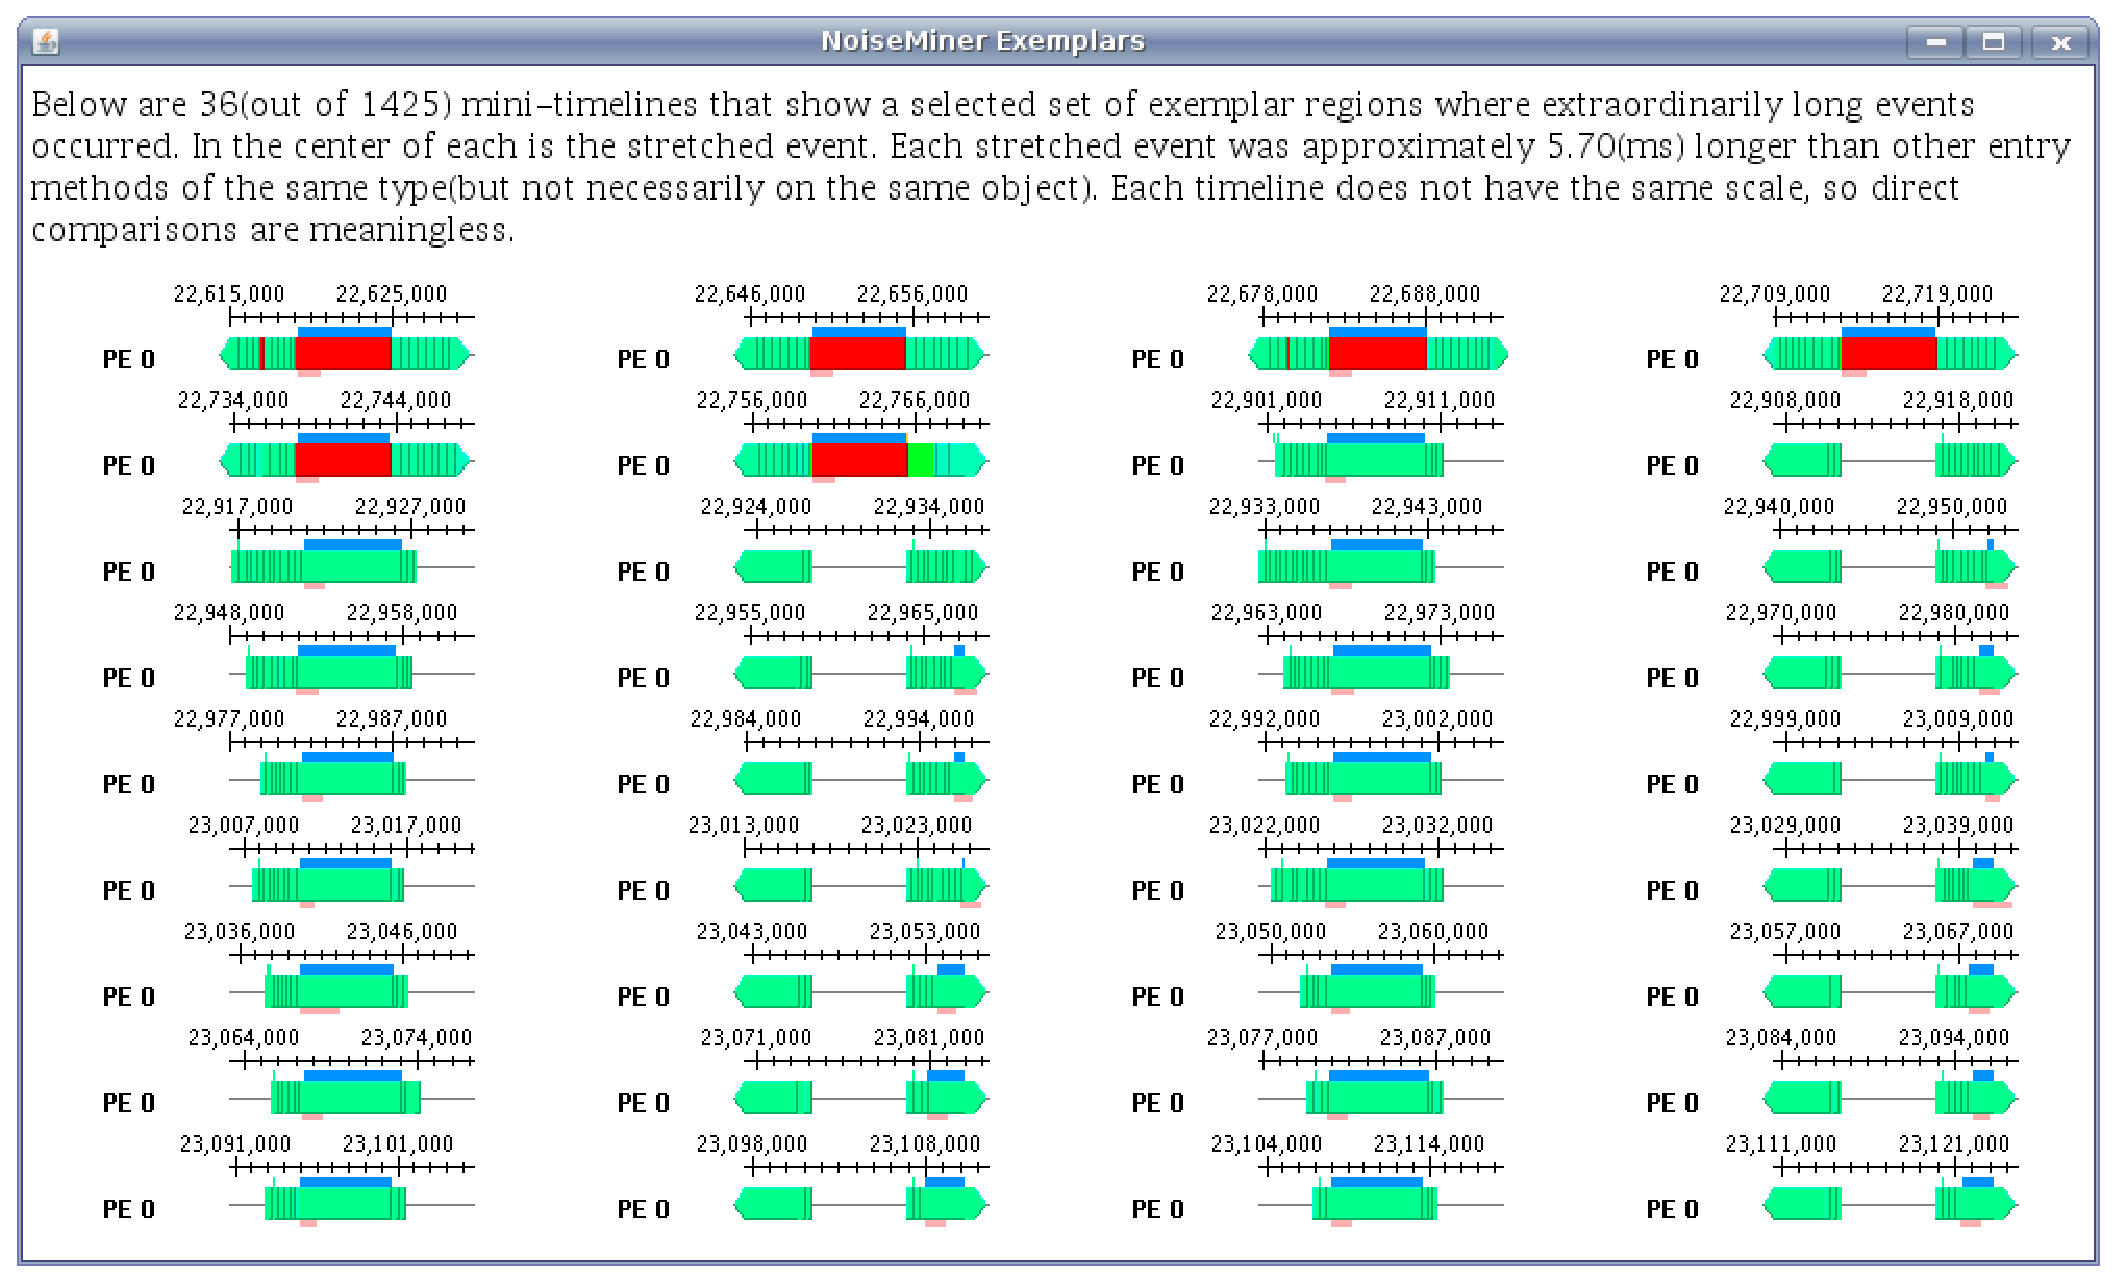
\includegraphics[width=6.0in]{fig/NoiseMiner2}
\caption{NoiseMiner noise component view showing miniature timelines for 
one of the noise components.\label{noiseminer2} }
\end{figure}

The NoiseMiner view (see figure \ref{noiseminer1} and
\ref{noiseminer2}) displays statistics about abnormally long entry
methods. Its purpose is to detect symptoms consistent with
\textit{Operating System Interference} or \textit{Compuatational
Noise} or \textit{Software Interference}. The abnormally long events
are filtered and clustered across multiple dimensions to produce a
concise summary. The view displays both the duration of the events as
well as the rate at which they occur. The initial dialog box allows a
selection of processors and a time range. The user should select a
time range that ignores any startup phase where events have chaotic
durations. The tool makes only a single pass through the log files
using a small bounded amount of memory, so the user should select as
large time range as possible.
 
The tool uses stream mining techniques to produce its results by making only one pass through the input data while using a limited amount of memory. This allows NoiseMiner to be very fast and scalable. 


The initial result window shows a list of zero or more noise
components. Each noise component is a cluster of events whose
durations are abnormally long. The noise duration for each event is
computed by comparing the actual duration of the event with an
expected duration of the event. Each noise component contains events
of different types across one or more processors, but all the events
within the noise component have similar noise durations. 

Clicking on the ``view'' button for a noise component opens a window similar to
figure \ref{noiseminer2}. This second window displays up to 36
miniature timelines, each for a different event associated with the
noise component.



NoiseMiner works by storing histograms of each entry method's
duration. The histogram bins contain a window of recent occurrences as
well as an average duration and count. After data stream has been
parsed into the histogram bins, the histogram bins are clustered to
determine the expected entry method duration. The histograms are
then normalized by the expected duration so that they represent the
abnormally stretched amounts for the entry methods. Then the histogram
bins are clustered by duration and across processors. Any clusters
that do not contribute much to the overall runtime are
dropped. 